\documentclass[11pt,letterpaper]{article}

\textwidth      =  6in
\textheight     =  8.25in
\oddsidemargin  =  18pt
\evensidemargin =  18pt
\topmargin      =  0.00in

\usepackage[utf8]{inputenc}
\usepackage[spanish]{babel}
\usepackage{amsmath}
\usepackage{amsfonts}
\usepackage{amssymb}
\usepackage{graphicx}
\graphicspath{{img/}}

\title{Título del trabajo}
\author{Autor 1\\ Autor Dos}

\begin{document}
\pagestyle{empty}
\begin{minipage}{.15\textwidth}
	
\includegraphics[scale=.22]{uv.eps}
\end{minipage}
\begin{minipage}{.7\textwidth}
\centering
{\huge \sc Universidad Veracruzana}\\
{\LARGE \sc Facultad de Matemáticas}
\end{minipage}
\begin{minipage}{.15\textwidth}
	\begin{flushright}
		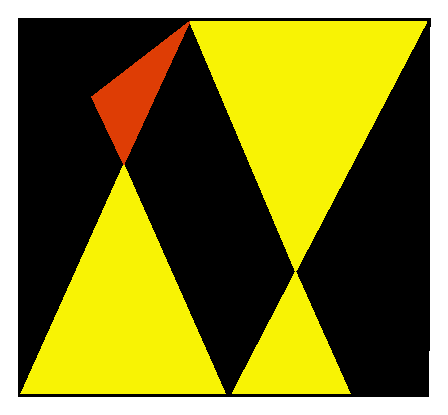
\includegraphics[scale=.22]{matematicas.eps}
	\end{flushright}
\end{minipage}

\vspace{.7cm}
\begin{center}
{\huge \bf
	Título del trabajo
}
\\[1.5cm]
{ \Huge
	T A R E A
}
\\[1.5cm]

{ \large
	Que para pasar la materia
}
\\[.5cm]
{ \LARGE \bf
	Temas Selectos de Matemáticas Divertidas
}
\\[1cm]
Presentan los siguientes\\[1cm]
{ \Large
I N T E G R A N T E S:
}\\
{ \LARGE \bf
	Autor Uno\\
	Autor Dos
}\\[1cm]
{ \Large
CATEDRÁTICO:
}\\
{ \LARGE \bf
	Homero Simpson
}
\end{center}
\vspace{1.5cm}
\begin{minipage}{.5\textwidth}
\centering
Xalapa, Veracruz
\end{minipage}
\begin{minipage}{.5\textwidth}
\centering
30 de febrero de 2019
\end{minipage}

%-----------------%
\pagebreak
\pagestyle{plain}

%
% Aquí iría el resto del contenido del documento
%

\end{document}
